	              
% --------------------------------------------------------------
% This is all preamble stuff that you don't have to worry about.
% Head down to where it says "Start here"
% --------------------------------------------------------------
 
\documentclass[11pt]{article}
\usepackage{ulem}
\usepackage[margin=1in]{geometry} 
\usepackage{graphicx}
\usepackage{amsmath,amsthm,amssymb} 
\newcommand{\N}{\mathbb{N}}
\newcommand{\Z}{\mathbb{Z}}
\DeclareMathOperator*{\argmax}{arg\,max}
\newenvironment{theorem}[2][Theorem]{\begin{trivlist}
\item[\hskip \labelsep {\bfseries #1}\hskip \labelsep {\bfseries #2.}]}{\end{trivlist}}
\newenvironment{lemma}[2][Lemma]{\begin{trivlist}
\item[\hskip \labelsep {\bfseries #1}\hskip \labelsep {\bfseries #2.}]}{\end{trivlist}}
\newenvironment{exercise}[2][Exercise]{\begin{trivlist}
\item[\hskip \labelsep {\bfseries #1}\hskip \labelsep {\bfseries #2.}]}{\end{trivlist}}
\newenvironment{reflection}[2][Reflection]{\begin{trivlist}
\item[\hskip \labelsep {\bfseries #1}\hskip \labelsep {\bfseries #2.}]}{\end{trivlist}}
\newenvironment{proposition}[2][Proposition]{\begin{trivlist}
\item[\hskip \labelsep {\bfseries #1}\hskip \labelsep {\bfseries #2.}]}{\end{trivlist}}
\newenvironment{corollary}[2][Corollary]{\begin{trivlist}
\item[\hskip \labelsep {\bfseries #1}\hskip \labelsep {\bfseries #2.}]}{\end{trivlist}}
 \usepackage{amsmath}
\usepackage{float}
 \floatplacement{figure}{H}
\begin{document}
 
% --------------------------------------------------------------
%                         Start here
% --------------------------------------------------------------
 
%\renewcommand{\qedsymbol}{\filledbox}
 
\title{CS 498: Project Final Report}%replace X with the appropriate number
\author{Adit Krishnan, UIN: 659913017, Net ID: aditk2 , Aravind Sankar, UIN: 671514664, Net ID: asankar3 \\} %if necessary, replace with your course title
\maketitle


\section{Introduction}
We address the task of discovering social circles in a user's ego network in this project. In addition to the baseline algorithms reported in the mid-term submission, we implement two algorithms for solving this problem. The first algorithm CESNA \cite{cesna} is a state of the art technique for detecting overlapping communities in a social network. We provide a best-effort implementation and report the results that we obtain. The second algorithm that we present here is our own model. We draw motivation from some ideas of existing techniques and our analysis of the datasets \cite{SNAP dataset}. 
In the next section, we provide a very brief description of the main idea behind CESNA. 
After that, we describe our proposed model in detail. Finally, we present the results of the two algorithms on the facebook ego-network dataset.

\section{Algorithm 1 - CESNA}
This paper proposes a probabilistic model for generating network topology and node attributes. They assume that each node in the network has a community membership which determines the edges observed in the network. Each community also has a relevance score with respect to each attribute. The community memberships along with attribute specific relevance score for each community are assumed to generate the observed network and attributes. They develop a gradient ascent algorithm to optimize their likelihood function.
\section{Algorithm 2 - Our model}
We first provide the main motivation behind the design of our model.
\subsection{Motivation}
We propose our model by drawing the basic idea of community memberships for each node from CESNA. However, we aim to simplify the network and attribute generation process and improve it using insights that we obtain from our dataset. First, we analyzed the ground truth communities in the given dataset to determine the edge density for each community. In Table 1, we show the mean value of density in each ego-network, along with the standard deviation. We can clearly see that there is a significant variation in the density of the ground truth communities. This shows that effect of edge formation due to each community is different and depends on the density of the community. We capture this explicitly in our model by allowing each community to have a different influence in edge formation.  \\[3pt]

The second insight is that node attributes in ego-networks tend to be very sparse and noisy. This means that explicitly modeling the generation of node attributes based on community memberships could lead to poor detected communities. Instead, we use the node attributes to capture the profile similarity between a pair of users, which is now used to guide the formation of edges in a network based on community memberships of each node. This also has an added benefit in that the complexity of the model is reduced greatly as we only model the likelihood of the observed edges in the network. To summarize, we model the likelihood of observing the network edges based on community memberships of each node, community density and node attributes. We define a likelihood function to capture this idea and propose a parallel optimization algorithm to infer the parameters of our model. We find that our model is much faster than CESNA (our implementation) in practice.
Next, we provide a formal description of our model. 

\subsection{Model formulation}
Given an undirected graph $G(V,E)$ with binary node attributes $X$,  the goal is to detect $C$ communities that could be overlapping. For now, we assume that the number of communities $C$ is given.  We describe the procedure to automatically find the best value of $C$ later.
We assume that there are $N$ nodes in the network $G$ and each node has $K$ attributes. We denote the network by $G$, and attributes by $X$.
Each node has a binary attribute vector denoted by $\mathbf{X_u}$ of size $K$,  
where $\mathbf{X_u} (k) = 1$ indicates the presence of attribute $k$ for node $u$ in the network. In addition to these basic observed variables, we have node community memberships $F$ and community density weights $W$. For community memberships $F$, we assume that each node $u$ has a non-negative affiliation weight $F_{uc}$ to community $c$. Each community has a non-negative weight $W_c$ which represents the density of the community. First we describe how similarity of two users is modeled using their node attributes. 

\subsubsection*{User similarity}
We model profile similarity of a pair of users $(u,v)$ using their node attributes. We use the cosine similarity to model this similarity as below : 
\[ sim_{uv} = \frac{\mathbf{X_u} \textbf{.} \mathbf{X_v} }{\| \mathbf{X_u}\| \|  \mathbf{X_v} \|}\]
This profile similarity will be used in combination user community memberships to model the likelihood of observing the network. Next, we describe a generative process of observing the links in the network.
\subsubsection*{Link generation}
In this section, we  describe how network structure depends on the different factors  outlined earlier and provide a mathematical formulation of the same.  First, we describe the effect of node community memberships.
Node community affiliations positively influence the likelihood that a pair of nodes is connected. The degree of influence depends on the communities that the pair of nodes belong to. Each community influences the link probability independently but proportional to the density of the community. Using these intuitions, we model this influence of community memberships as proportional to $F_{uc} F_{vc} W_c$ for a pair of users $(u,v)$ w.r.t. community $c$.
Next, the link probability between a pair of nodes also depends on their user profile similarity, which is modeled as proportional to $sim_{uv}$.  We combine the two effects to model the probability that two nodes $u, v$ belonging to a community $c$ are connected as : 

\[ P_{uv} (c) = 1 - \exp(- \left\lbrace \alpha F_{uc}. W_c. F_{vc} + (1 - \alpha) \frac{sim_{uv}}{C} \right\rbrace ) \]

Here, $\alpha$ is a hyper-parameter that controls the effect of the two factors in modeling the link probability. We assume that each community $c$ connects nodes $u,v$ independently with probability $P_{uv} (c)$.  For $u$ and $v$ to be connected, it must be connected by at least one community which gives a link generation probability $P_{uv}$ as : 
\begin{align*}
P_{uv} &=  1 - \prod_{c=1}^C (1 - P_{uv}(c) )  \\
 &=1 - \prod_{c=1}^C \exp(- \left\lbrace \alpha F_{uc}. W_c. F_{vc} + (1 - \alpha) \frac{sim_{uv}}{C} \right\rbrace ) \\
 &= 1 - \exp( -\sum\limits_{c=1}^C \left\lbrace \alpha F_{uc}. W_c. F_{vc} + (1 - \alpha) \frac{sim_{uv}}{C} \right\rbrace)  \\
 &= 1 - \exp( - ( \alpha \mathbf{F_u^{T}} \mathbf{W} \mathbf{F_v} + (1 - \alpha) sim_{uv}))
\end{align*}
Here, $\mathbf{F_u}$ denotes the vector of community memberships (of size $C$) for node $u$. $\mathbf{W}$ is a diagonal matrix of size $C \times C$ with entries from $W$.
This defines the link generation probability in the network. We assume a Multi-Bernoulli process for link generation i.e. each link $(u,v)$ is modeled by a Bernoulli distribution with parameter $P_{uv}$.  This completes the basic formalism of our model. We can clearly observe that the different factors mentioned earlier are captured in modeling this link generation probability. In the section, we describe how to infer communities by formulating a likelihood function that we optimize using gradient ascent. 

\subsection{Community Inference}
In this section, we describe how we detect network communities by estimating the model parameters from the given data. We aim to infer the values of latent variables $F$ and $W$ based on the observed network and attributes. We note that though the attributes are also observed, we only model the likelihood of the network structure as the attributes are captured in the link generation probability. 
We define the likelihood of the observed network $G$ as  $P(G \mid F, W, X)$ given by : 

\[ P(G \mid F, W, X)  = \prod_{u, v \in E} P_{uv} \prod_{u,v \notin E} (1 - P_{uv}) \]

To find the optimal $\hat{F}$ and $\hat{W}$,  we optimize the log-likelihood of the observed network as : 
\begin{align*}
 \mathcal{L}  &= \log P(G \mid F, W, X)  \\
 &= \sum\limits_{u,v \in E} \log \Big( 1 - \exp( - ( \alpha \mathbf{F_u^{T}} \mathbf{W} \mathbf{F_v} + (1 - \alpha) sim_{uv})) \Big) - \sum\limits_{u, v \notin E} ( \alpha \mathbf{F_u^{T}} \mathbf{W} \mathbf{F_v} + (1 - \alpha) sim_{uv})) \\
&= \sum\limits_{u,v \in E} \log \Big( 1 - \exp( - \psi(u,v) \Big) - \sum\limits_{u, v \notin E} \psi(u,v) \\[4pt]
& \text{ where }  \psi(u,v) =  \alpha \mathbf{F_u^{T}} \mathbf{W} \mathbf{F_v} + (1 - \alpha) sim_{uv} = \alpha \sum\limits_{c=1}^C F_{uc} W_c F_{vc} + (1 - \alpha) sim_{uv}\\
\end{align*}


Thus, the optimization problem that we aim to solve is: 
\[ \hat{F}, \hat{W} = \argmax_{F, W \geq 0} \mathcal{L} \]
To solve this optimization problem, we use gradient ascent. We can easily show that the above likelihood function is concave in both $F$ and $W$. Since we impose non-negativity constraints on $F$ and $W$, we compute gradient updates for each variable and then project onto to space of non-negative real numbers $[0, \infty)$. \\
  
\subsubsection*{Gradient update for F}
In order to update the community memberships $F_u $of a node $u$, we fix all other parameters (the memberships of all other nodes and $W$) and then compute the gradient update for $u$. Thus, the sub-problem that we solve for a node $u$ is given by: 
\begin{align*}
\mathcal{L} (F_u) = \sum\limits_{v \in N(u)} \log (1 - \exp(- \psi(u,v)))  - \sum\limits_{v \notin N(u)} \psi(u,v)
\end{align*}
Here, $N(u)$ denotes the set of all neighbors of node $u$ in the network $G$.
We now derive the gradient update rule for each $F_{uc}$, which is given as : 
\begin{align*}
\frac{\partial \mathcal{L}}{F_{uc}} &= \sum\limits_{v \in N(u) } \alpha F_{vc} W_c \frac{\exp(- \psi(u,v))}{1 - \exp(-\psi(u,v))} - \sum\limits_{v \notin N(u)} \alpha F_{vc} W_c  \\ 
&= \sum\limits_{v \in N(u) } \alpha F_{vc} W_c \frac{\exp(- \psi(u,v))}{1 - \exp(-\psi(u,v))}  - \alpha \left\lbrace \sum\limits_{v \in V} F_{vc} W_c - F_{uc} W_c - \sum\limits_{v \in N(u)} F_{vc} \right\rbrace
\end{align*}

We obtain the first equation by taking the gradient of $\mathcal{L}$ w.r.t $F_{uc}$. We can simplify the summation over all non-neighbors of $u$ by re-writing it as function of just the neighbors of $u$, since the term $\sum\limits_{v \in V} F_{vc}$ can be computed in advance. The update equation for $F_{uc}$ now becomes : 
\begin{equation}
 F_{uc}^{n+1} =  \max \Big(0, F_{uc}^n  + \eta_u \frac{\partial \mathcal{L}}{F_{uc}^n}\Big) 
\end{equation}
In this equation, $\eta_{u}$ is the learning rate for the node $u$, which is estimated using backtracking line-search \cite{boyd} for performing the gradient updates of node $u$. We note here that the gradient equation (1) here lends itself to easy parallelism. Specifically, we can perform the gradient updates for each node $u$ in parallel, which will leads to great speedup. 
\subsubsection*{Gradient update for W}
The gradient update for $W$ is derived in a very similar manner to $F$. We keep the community memberships of all nodes ($F$) fixed when we perform the gradient updates for $W$. Thus, we get the gradient w.r.t $W_c$ as : 

\begin{align*}
\frac{\partial \mathcal{L}}{W_{c}}  = \sum\limits_{u,v \in E}  \alpha F_{uc} F_{vc} \frac{\exp(- \psi(u,v))}{1 - \exp(-\psi(u,v))} -  \alpha \left\lbrace \sum\limits_{u, v \notin E} \alpha F_{uc} F_{vc} \right\rbrace
\end{align*}
The gradient update for $W_c$ is given by : 

\begin{equation}
W_{c}^{n+1} =  \max \Big(0, W_{c}^n  + \eta_w \frac{\partial \mathcal{L}}{W_{c}^n}\Big) 
\end{equation}
In this case also, we can capture gradients  for each community is parallel.  The learning rate $\eta_w$ is again learned using line search. \\[3pt]
The gradient ascent algorithm is performed by alternatively updating $F$ and $W$ in each iteration.  We stop when the relative change in likelihood is less than 0.001 \% or if 1000 iterations has been reached. We provide a parallel implementation of both our algorithm and CESNA in Java. 
\subsubsection*{Detecting community assignments}
The gradient ascent algorithm will give us community memberships for each node $u$ in the network. We use an idea similar to what is used by CESNA to detect communities. To determine if node $u$ belongs to community $c$, we require that $F_{uc}$ is greater than a threshold $\delta_c$ for community $c$. We set $\delta_c$ so that node $u$ belongs to community $c$ if $u$ is connected to other members of $c$ with an edge probability greater than $1/N$. In doing so, we ignore the contribution of attributes to the edge probability. 
We determine $\delta_c$ as : 

\[ 1 - \exp(1 - \delta_c^2 W_c) \geq \frac{1}{N} \]
This gives us :
$$\delta_c = \sqrt{\frac{\log(\frac{N}{N-1})}{W_c}}$$

\subsubsection*{Choosing the best number of communities}
In order to automatically find the best number of communities $C$, we remove $10 \%$ of the edges from the network to create a hold-out set. Then, we vary $C$ in a range from 5 to 15 and fit the remaining network using our model.  We evaluate the likelihood of the hold-out set using our estimated model. The value of $C$ that gives us maximum likelihood on the held-out set is chosen as the number of communities. \\[5pt]
In our model, we have only one hyper-parameter $\alpha$ which determines the trade-off between user profile similarity and node community memberships. It is set to 0.5 by default. 

\subsubsection*{Initial community memberships}
TODO - conductance etc.

\section{Experimental Evaluation}
\subsection{Setup}
\subsection{Running Time}
\subsection{Quality}
We evaluate the quality of the communities using the evaluation metric proposed in CESNA given by : 
\[ \frac{1}{2 |C^{*}|} \sum\limits_{C_i^{*} \in C^{*}} \max_{C_j \in C} \delta (C_i^{*}, C_j) + \frac{1}{2 |C|} \sum\limits_{C_j \in C} \max_{C_i^{*} \in C^{*}} \delta (C_i^{*}, C_j) \]

Here, $C$ denotes the  predicted communities and $C^{*}$ the original ground truth communities. $\delta(C_i^{*}, C_j)$ is a similarity measure between the communities $C_i^{*}$ and $C_j$ which we assume to be the Jaccard similarity. The performance of our model and CESNA based on this metric, are shown below :

\begin{table}[H]
\begin{center}
\begin{tabular}{|c|c|c|}
\hline
\textbf{Graph} & \textbf{CESNA} & \textbf{Our Model} \\ \hline
Graph 0 & 0.1782 & 0.1837 \\ \hline
Graph 107 & 0.2423 & 0.25264 \\ \hline
Graph 348 & 0.3952 & 0.40088 \\ \hline
Graph 414 & 0.5203 & 0.5278 \\ \hline
Graph 686 & 0.3577 & 0.35028 \\ \hline
Graph 698 & 0.5349 & 0.576 \\ \hline
Graph 1684 & 0.3191 & 0.36822 \\ \hline
Graph 1912 & 0.2696 & 0.32478 \\ \hline
Graph 3437 & 0.101 & 0.10666 \\ \hline
Graph 3980 & 0.3375 & 0.32564 \\ \hline
\end{tabular}
\end{center}
\caption{Performance comparison of our model and CESNA on the Facebook dataset}
\end{table}

The plot depicting the comparison of the two algorithms is shown below.
\begin{figure}[H]
\begin{center}
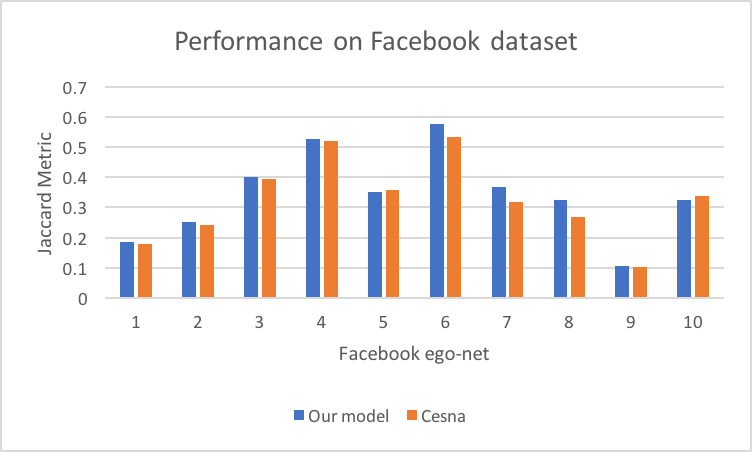
\includegraphics[scale=1]{plot.png}
\caption{Histogram showing the performance of our model and CESNA on different graphs}
\end{center}
\end{figure}
\begin{thebibliography}{3}
\bibitem{boyd}
Boyd, Stephen, and Lieven Vandenberghe. Convex optimization. Cambridge university press, 2004.
\bibitem{SNAP}
Leskovec, Jure. "Stanford network analysis package (snap)." URL http://snap. stanford. edu (2013).
\bibitem{SNAP dataset}
Leskovec, Jure, and Andrej Krevl. "SNAP Datasets: Stanford large network dataset collection, June 2014." URL: http://snap. stanford. edu/data (2014).
\bibitem{facebook dataset}
McAuley, Julian J., and Jure Leskovec. "Learning to Discover Social Circles in Ego Networks." NIPS. Vol. 2012. 2012.
\bibitem{cesna}
Yang, Jaewon, Julian McAuley, and Jure Leskovec. "Community detection in networks with node attributes." 2013 IEEE 13th International Conference on Data Mining. IEEE, 2013.
\bibitem{plsa}
Hofmann, Thomas. "Probabilistic latent semantic indexing." Proceedings of the 22nd annual international ACM SIGIR conference on Research and development in information retrieval. ACM, 1999.
\bibitem{lda}
Blei, David M., Andrew Y. Ng, and Michael I. Jordan. "Latent dirichlet allocation." Journal of machine Learning research 3.Jan (2003): 993-1022.
\bibitem{l1}
 L. Akoglu, H. Tong, B. Meeder, and C. Faloutsos. PICS: Parameter-free
Identification of Cohesive Subgroups in Large Attributed Graphs. SDM
’12, 2012.
\bibitem{l2}
M. Ester, R. Ge, B. Gao, Z. Hu, and B. Ben-Moshe. Joint Cluster
Analysis of Attribute Data and Relationship Data: the Connected kCenter
Problem. In SDM ’06, 2006.
\bibitem{johnson}
Johnson, Stephen C. "Hierarchical clustering schemes." Psychometrika 32.3 (1967): 241-254.
\end{thebibliography}

\end{document}